\chapter{\babTiga}
\label{bab:3}



\noindent\todo{
	jabarin sih isinya mau gmna
}

\section{\f{Transformer}}

\begin{figure}
	\centering
	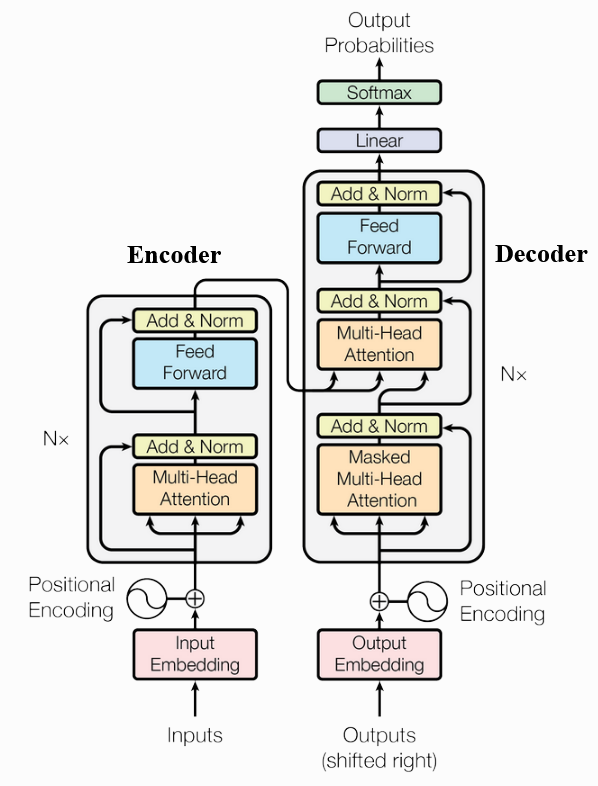
\includegraphics[width=0.7\linewidth]{assets/pics/transformers_seq.png}
	\caption{Arsitektur \f{transformer} untuk mesin translasi neural. Arsitektur terdiri dari \f{encoder} dan \f{decoder} yang terdiri dari beberapa blok \citep{transformerori}.}
	\label{fig:transformer}
\end{figure}

\f{Transformers} merupakan Arsitektur \f{deep learning} yang pertama kali diperkenalkan oleh \cite{transformerori}. Awalnya Transformers merupakan model \f{sequance to sequance} yang diperuntukkan untuk permasalahn mesin translasi neural (\f{neural machine translation}). Namun, sekarang \f{transformers} juga digunakan untuk permasalahan pemrosesan bahasa alami lainnya. model-model yang menjadi \f{state of the art} permasalahan pemrosesan bahasa alami biasanya menggunakan arsitektur \f{transformers}.

Berbeda dengan arsitektur mesin translasi terdahulu \citep{RNNseq2seq}, transformers tidak mengunakan \f{recurrent neural network} (RNN) atau \f{convolutional neural network} (CNN), melainkan transformers adalah model \f{feed foward network} yang dapat memproses seluruh \f{input} pada barisan secara paralel. Untuk menggantikan kemampuan RNN dalam mempelajari ketergantungan antar \f{input} yang berurutan dan kemampuan CNN dalam mempelajari fitur lokal, transformers bergantung pada mekanisme \f{attention}.

Terdapat tiga jenis \f{attention} yang digunakan dalam model \f{transformers} \citep{transformerori}:

\begin{enumerate}
	\item \f{Encoder self-attention} menggunakan barisan \f{input} yang berupa kalimat sebagai masukan untuk menghasilkan barisan representasi kontekstual (vektor) dari \f{input}. Setiap representasi token tersebut memiliki ketergantungan dengan token lainnya dalam urutan masukan.
	\item \f{Decoder self-attention} menggunakan barisan \f{target} yang berupa kalimat terjemahan parsial sebagai masukan untuk menghasilkan barisan representasi kontekstual (vektor) dari \f{target}. Setiap representasi token tersebut memiliki ketergantungan dengan token sebelumnya dalam urutan masukan.
	\item \f{Decoder-encoder attention} menggunakan barisan representasi kontekstual dari \f{input}, dan barisan representasi kontekstual dari \f{target} untuk menghasilkan token berikutnya yang merupakan hasil prediksi dari model. barisan \f{target} yang digabung dengan token hasil prediksi tersebut akan menjadi barisan \f{target} untuk prediksi selanjutnya.
\end{enumerate}

\subsection{\f{Attention}}

\begin{figure}
	\centering
	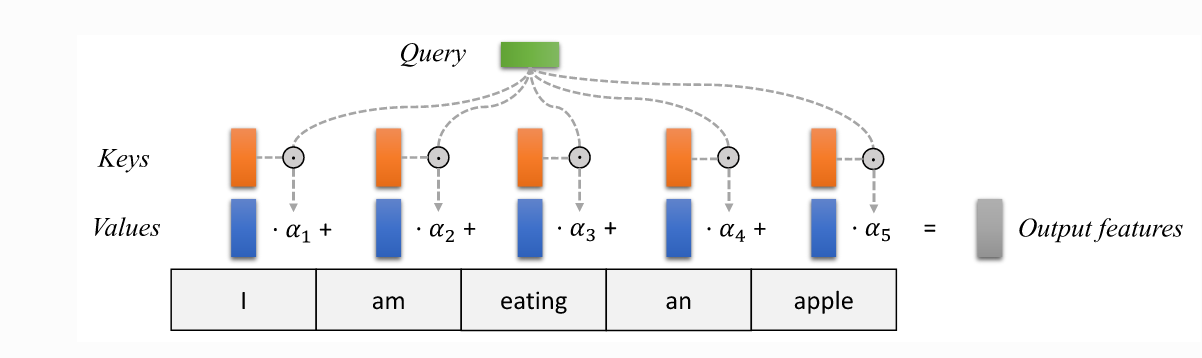
\includegraphics[width=0.7\linewidth]{assets/pics/attention.png}
	\caption{Mekanisme \f{attention} \citep{lippe2022uvadlc}.}
	\label{fig:attention}
\end{figure}

Mekanisme \f{attention} menggambarkan rata-rata terbobot dari barisan elemen dengan bobot yang dihitung secara dinamis berdasarkan kueri masukan dan Kunci elemen. Tujuannya adalah untuk mengambil rata-rata dari fitur beberapa elemen. Namun, daripada memberi bobot setiap elemen secara merata, kita ingin memberi bobot tergantung pada "nilai" elemen tersebut. Dengan kata lain, kita ingin secara dinamis memutuskan elemen masukan mana yang ingin kita perhatikan lebih dari yang lain. Mekanisme \f{attention} biasanya memiliki empat bagian yang perlu ditentukan:

\begin{enumerate}
	\item Kueri ($\mathbf{q}$): Kueri adalah vektor yang merepresentasikan apa yang ingin dicari dalam barisan elemen.
	\item Kunci ($\mathbf{k}$): Untuk setiap elemen dalam barisan, terdapat vektor yang disebut kunci. Vektor fitur ini secara kasar merepresentasikan apa yang ditawarkan elemen tersebut, atau kapan elemen tersebut menjadi penting. Kunci harus dirancang sedemikian rupa sehingga kita dapat mengidentifikasi elemen yang ingin kita perhatikan berdasarkan kueri.
	\item Nilai ($\mathbf{v}$): Untuk setiap elemen dalam barisan, terdapat vektor yang disebut nilai. vektor nilai ini yang ingin dirata-ratakan.
	\item Fungsi skor ($f_{\text{attn}}(\mathbf{q}, \mathbf{k})$): Fungsi skor memberikan bobot-bobot pada pada nilai berdasarkan kueri dan kunci. Fungsi skor dapat dihitung dengan berbagai cara, seperti cara sederhana berupa perkalian skalar atau jarak kosinus, dan dapat juga dihitung menggunakan fungsi skor yang lebih kompleks seperti \f{multi-layer perceptron} (MLP). \pic~\ref{fig:attention} memberikan gambaran dari mekanisme \f{attention}.
\end{enumerate}

\noindent\begin{align}
	\alpha_i &= \frac{\exp(f_{\text{attn}}(\mathbf{q}, \mathbf{k}_i))}{\sum_{j=1}\exp(f_{\text{attn}}(\mathbf{q}, \mathbf{k}_j))} \label{eq:attentionweight}\\
	\text{Output} &= \sum_{i=1} \alpha_i \mathbf{v}_i \label{eq:attentionoutput}
\end{align}

Biasanya, hasil fungsi skor diterapkan pada fungsi softmax untuk mendapatkan bobot yang dinormalisasi. Bobot tersebut kemudian digunakan untuk menghitung rata-rata terbobot dari nilai. \equ~\ref{eq:attentionweight} menujukkan bagaimana bobot dihitung, dan \equ~\ref{eq:attentionoutput} menunjukkan proses perhitungan rata-rata terbobot.

\subsubsection{\f{Self-Attention}}


\subsubsection{\f{Multi-Head Attention}}
\subsection{\f{Positional Encoding}}
\subsection{\f{Feed Forward Network}}
\subsection{Arsitektur \f{Transformer} Enkoder}

\section{\f{Bidirectional Encoder Representation from Transformer (BERT)}}
\subsection{model pralatih BERT}
\subsubsection{Tugas \f{Masked Language Model (MLM)}}
\subsubsection{Tugas \f{Next Sentence Prediction (NSP)}}
\subsection{IndoBERT}
\section{Arsitektur \bertcat~Untuk Pemeringkatan Teks}
\section{Arsitektur \bertdot~Untuk Pemeringkatan Teks}



